\chapter{Chance-Constraint Optimization with Kernel Approximation} \label{Technical Approach}

In this chapter, an approach is outlined that allows us to effectively reformulate the chance-constraint problem defined in section \ref{Problem Statement} using the samples generated using the method described in chapter \ref{Technical Background}.

In section \ref{Scenario Approach} a method was presented that allows us to reformulate the chance-constraints as a determinstic OCP. However, the final problem no longer contains the risk factor $\alpha$ which is why in this section a alternative approach is presented that allows us to has been lo, a method that enables us to generate a finite number of scenarios $\boldsymbol{\delta}^{[1:N]}$ was presented. These scenarios can be used to formulate an OCP to find an optimal $\boldsymbol{u}$ or a control law $\boldsymbol{\pi}$. In this section, a method to use maximum mean discrepancy (MMD) ambiguity sets and kernel approximation to reformulate the OCP is proposed.

\section{MMD ambiguity sets} \label{SubSec:MMD}

As the underlying data distribution $P$ in the constraints \eqref{constraints} is unknown, we first expand the them to their distributionally robust counterpart in order to allow for the use of scenarios as an approximation of the distribution. For this, we consider $P$ as the worst case distribution within a set $\mathcal{P}$ of plausible distributions, the so-called ambiguity set. This gives us the new constraints

\begin{equation} \label{wc constraints}
\inf\limits_{\tilde{P} \in \mathcal{P}}\tilde{P} \left[ \text{max}(\boldsymbol{h}(\boldsymbol{u}_{0:H},  \boldsymbol{x}_{0:H},  \boldsymbol{y}_{0:H})) \leq 0 \right] \geq 1 - \alpha.
\end{equation}

\begin{figure}
\centering
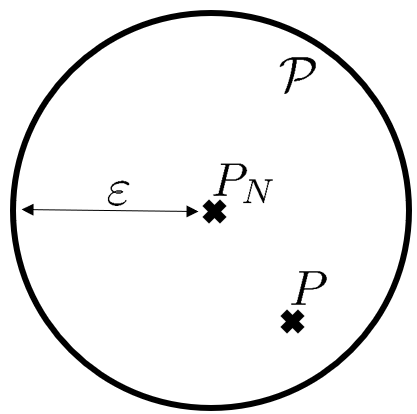
\includegraphics[width= .4\textwidth]{AmbiguitySetDrawing}
\caption{Ambiguity Set $\mathcal{P}$}
\label{AmbiguityPic}
\end{figure}

To construct the set $\mathcal{P}$, a similarity measure is needed to provide a concrete comparison between various distributions $\tilde{P}$. Maximum mean discrepancy (MMD) \cite{Arthur_12} is able to do that by using the norm of the difference between the kernel mean embeddings (KME) $|| \mu_Q - \mu_{Q'} ||^2_{\mathcal{H}}$ of two distributions $Q$ and $Q'$ as a metric between two distributions. The KME are given as $\mu_Q = \int k(x, \cdot) \text{d}x$ with $k(x, \cdot) \in \mathcal{H}$ being the feature map of the kernel function $k$. The metric can then be rewritten as 

\begin{equation} \label{MMD Kernel}
\text{MMD}(Q, Q') = \text{E}_{z,z' \sim Q}[k(z,z')] + \text{E}_{z,z' \sim Q'}[k(z,z')] - 2\text{E}_{z\sim Q, z' \sim Q'}[k(z,z')]
\end{equation}

The MMD-based ambiguity set $\mathcal{P}$ is then constructed as the set of distributions $\tilde{P}$ in an $\varepsilon$ radius centered around the empirical distribution $P_N$ which is given through the scenarios $\boldsymbol{\delta}^{[1:N]}$. This gives us the set

\begin{equation} \label{ambiguity set}
\mathcal{P} =  \left\{ P : \text{MMD} (P, P_N) \leq \varepsilon \right\}.
\end{equation}

The radius $\varepsilon$ is chosen through constructing a bootstrap MMD ambiguity set as described in \cite{Yassine_22} and is outlined in Algorithm \ref{alg:Bootstrap}. This procedure requires a number of bootstrap samples $B$ to be chosen, as well as confidence level $\beta$. It then utilizes kernels $k(\boldsymbol{\delta}^{[i]}, \boldsymbol{\delta}^{[j]}) \in \mathbb{R}$ to define the (biased) MMD estimator as 

\begin{equation} \label{ambiguity set approx}
\widehat{\text{MMD}} (\tilde{P}, P_N) = \sum_{i,j = 1}^N k(\boldsymbol{\delta}^{[i]}, \boldsymbol{\delta}^{[j]}) + k(\tilde{\boldsymbol{\delta}}^{[i]}, \tilde{\boldsymbol{\delta}}^{[j]}) - 2 k(\boldsymbol{\delta}^{[i]}, \tilde{\boldsymbol{\delta}}^{[j]})
\end{equation}

with $\tilde{\boldsymbol{\delta}}^{[n]}, n = 1,...,N$, denoting a bootstrap sample of $P_N$ where samples are drawn with replacement from $\boldsymbol{\delta}^{[1:N]}$. Finally, $\widehat{\text{MMD}} (\tilde{P}, P_N)$ is calculated for all $B$ bootstrap samples, the results are saved in list and $\varepsilon$ is chosen as the $\textit{ceil}(B \beta)$-th element of the sorted list. 


\begin{algorithm}
	\caption{Bootstrap MMD ambiguity set}
	\label{alg:Bootstrap}
	\hspace*{\algorithmicindent} \textbf{Input}: Scenarios $ \boldsymbol{\delta}^{[1:N]} $, Number of bootstrap samples $B$, Confidence level $\beta$ \\
	\hspace*{\algorithmicindent} \textbf{Output}: Gram matrix $\boldsymbol{K}$, Radius of MMD ambiguity set $\varepsilon$
	\begin{algorithmic}[1]
		\State $\boldsymbol{K} \gets \textit{kernel}(\boldsymbol{\delta}, \boldsymbol{\delta})$
		\For{$m = 1, \dots , B$}
			\State $I \gets N$ numbers from $\{1, \dots N \}$ with replacement
			\State $K_x \gets \sum_{i,j = 1}^N K_{ij};$
			\State $K_y \gets \sum_{i,j \in I} K_{ij};$
			\State $K_{xy} \gets \sum_{j \in I} \sum_{i = 1}^N K_{ij}$;
			\State MMD$[m] \gets \frac{1}{N^2} \left( K_x + K_y - 2 K_{xy} \right) ;$
		\EndFor
		\State MMD $\gets$ \textit{sort}(MMD)
		\State $\varepsilon \gets$ MMD$\left[ \textit{ceil} (B \beta) \right]$
	\end{algorithmic}
\end{algorithm}

\section{Constraint Reformulation} \label{Constraint Reformulation}

With a given MMD ambiguity set $\mathcal{P}$, the feasible set of each constraint \ref{risk constraints} is given as

\begin{equation} \label{feasible set}
	Z :=  \left\{ \boldsymbol{u}_{0:H} \in \mathcal{U}^{H+1} : \inf\limits_{P \in \mathcal{P}}P \left[ \tilde{h}(\boldsymbol{u}_{0:H},  \boldsymbol{\delta}) \leq 0 \right] \geq 1 - \alpha \right\}.
\end{equation}

with $\tilde{h}(\boldsymbol{u}_{0:H},  \boldsymbol{\delta}) =  \text{max}(\boldsymbol{h}(\boldsymbol{u}_{0:H},  \boldsymbol{x}_{0:H},  \boldsymbol{y}_{0:H}))$.

We can now use the ambiguity set $\mathcal{P}$ defined in Sec. \ref{SubSec:MMD} with the radius $\varepsilon$ and the kernel matrix $\boldsymbol{K}$ to reformulate the feasible set. The matrix $\boldsymbol{K}$ contains the kernels of all possible combinations of samples. By following the steps described in \cite{Yassine_22}, we can obtain the new reformulated feasible set as

\begin{subequations}
  \begin{empheq}[right = \empheqrbrace, left= Z_i \coloneqq \empheqlbrace \boldsymbol{u}_{0:H} \in \mathcal{U}^{H+1} :]{align}
    & g_0 + \frac{1}{N}\sum_{n = 1}^N (\boldsymbol{K}\boldsymbol{\gamma})_n + \varepsilon \sqrt{\boldsymbol{\gamma}^\text{T}\boldsymbol{K}\boldsymbol{\gamma}} \leq t \alpha \\
    & [\tilde{h}(\boldsymbol{u}_{0:H},  \boldsymbol{\delta}^{[n]}) + t]_+ \leq g_0 + (\boldsymbol{K}\boldsymbol{\gamma})_n, \; n = 1,...,N \\
    & g_0 \in \mathbb{R}, \boldsymbol{\gamma} \in \mathbb{R}^N, t \in \mathbb{R}
  \end{empheq}
\end{subequations}

where $[\cdot]_+ = \text{max}(0, \cdot)$ denotes the max operator. The new set also contains new variables that have to be taken into account when solving the OCP. The variables $g_0$, $\gamma$ and $t$ are additional degrees of freedom can be incorperated into the OCP. The former are parameters of the RKHS function that was used to transform the problem into a kernel machine learning problem while $t$ has been introduced as a way to relax the risk factor $\alpha$.

We can then use this feasible set to formulate the OCP as

\begin{subequations}
\begin{align}
\begin{split}
\min\limits_{\boldsymbol{u}_{0:H},\boldsymbol{\gamma}, g_0, t' }  J_H(\boldsymbol{u}_{0:H})
\end{split}\\
\begin{split}
\text{s.t.}\; &\forall n = 1,...,N, \;  \forall t = 0,1,...,H
\end{split}\\
\begin{split}\label{systemc1}
&\boldsymbol{x}_{t+1}^{[n]} = \boldsymbol{f}_{\boldsymbol{\theta}^{[n]}} \left( \boldsymbol{x}_{t}^{[n]} , \boldsymbol{u}_t \right) + \boldsymbol{v}_{t}^{[n]}
\end{split}\\
\begin{split}\label{systemc2}
&\boldsymbol{y}_{t} = \boldsymbol{g}_{\boldsymbol{\theta}^{[n]}} \left( \boldsymbol{x}_{t}^{[n]}, \boldsymbol{u}_t \right) + \boldsymbol{w}_{t}^{[n]}
\end{split}\\
\begin{split}\label{systemc3}
 &\boldsymbol{u}_{0:H} \in Z(\boldsymbol{\gamma}, g_0, t')
\end{split}
\end{align}
\label{OCP_final}
\end{subequations}

As described in Sec. \ref{Problem Statement}, we are minimizing a cost function $J_H$. The system dynamics are included through the constraints \eqref{systemc1} and \eqref{systemc2} and must be fulfilled for all scenarios as well. Lastly, the input $u_{0:H}$ is restricted to the feasible set $Z$ in \eqref{systemc3} which is defined by the optimization variables $\boldsymbol{\gamma}$, $g_0$ and $t'$.

The optimization problem \eqref{OCP_final} is deterministic and can be solved with well known methods. 




